\documentclass[pdflatex,sn-mathphys-num]{sn-jnl}

\usepackage{graphicx}
\usepackage{booktabs}
\usepackage{array}
\usepackage{url}
\usepackage{amsmath,amssymb,amsfonts}
\usepackage{xcolor}
\usepackage{multirow}
\usepackage{textcomp}
\usepackage{threeparttable}
\usepackage{rotating}
\usepackage{appendix}
\usepackage{mathrsfs}

\raggedbottom

\begin{document}

\title[Pilot Study for Traditional Mongolian Archive Layout Analysis]{A Pilot Study for Text-Column Detection and Reading-Order Evaluation in Traditional Mongolian Historical Archives}

\author[1]{\fnm{Lanying} \sur{Liang}}\email{389647973@qq.com}
\author*[2]{\fnm{Yuefeng} \sur{Liu}}\email{liuyuefeng@imust.edu.cn}

\affil[1]{\orgdiv{Archives}, \orgname{Inner Mongolia University of Science and Technology}, \orgaddress{\city{Baotou}, \postcode{014010}, \state{Inner Mongolia}, \country{China}}}
\affil*[2]{\orgdiv{School of Digital and Intelligent Industry (School of Cyber Science and Technology)}, \orgname{Inner Mongolia University of Science and Technology}, \orgaddress{\city{Baotou}, \postcode{014010}, \state{Inner Mongolia}, \country{China}}}

\abstract{Traditional Mongolian historical archives pose a challenging page-level document analysis problem because the script is vertically written, cursive, low-resource, and frequently degraded by aging paper, ink variation, seals, scanning rotation, and heterogeneous archive sources. Since expert transcription of handwritten traditional Mongolian columns is expensive and currently unavailable, this work focuses on an upstream stage for archival OCR: text-column detection and reading-order recovery. We construct a page-level annotation protocol that records text-column bounding boxes, ignored noise regions, orientation metadata, and reading order. We compare classical rule-based extraction, YOLOv8n, and a COCO-pretrained Faster R-CNN MobileNet detector, and evaluate reading-order recovery on the matched detections. On an expanded 54-page test set, YOLOv8n improves the project-level IoU@0.5 F1 score from 0.722 for the heuristic baseline to 0.875 and achieves 0.887 reading-order accuracy on matched columns, while Faster R-CNN reaches 0.866 F1 after fine-tuning. However, page-level full success remains low (0.074 for YOLOv8n), so the system should be interpreted as a candidate crop generator rather than a fully automatic page-level OCR preprocessing system. We provide a crop-export-ready interface, but explicitly do not report CER/WER because column-level expert transcripts are not yet available. The study therefore provides a pilot study and evaluation package for subsequent traditional Mongolian archival OCR research, subject to archive-image access restrictions.}

\keywords{historical document analysis, traditional Mongolian archives, text column detection, reading order recovery, low-resource document analysis}

\maketitle

\section{Introduction}
Full-page recognition of traditional Mongolian historical archives requires more than a recognizer trained on isolated text lines. The input pages often contain many vertical handwritten columns, irregular spacing, red seals, page borders, paper stains, and inconsistent scan orientations. If the text columns are not localized and ordered reliably, downstream OCR modules receive incomplete or misordered crops, making page-level transcription unreliable.

In the present stage, expert transcription of handwritten traditional Mongolian archive columns is not available. Rather than reporting unverifiable OCR accuracy, this paper focuses on the upstream page-layout problem that can be rigorously evaluated with bounding-box and reading-order annotations. This setting is practically important: page-level layout annotations are much cheaper to obtain than full textual transcription, and they form the necessary bridge between scanned archive images and later recognition modules.

Our contributions are threefold. First, we define a page-level annotation protocol for traditional Mongolian archives, including TextColumn boxes, Ignore regions, orientations, and reading order. Second, we provide a pilot evaluation workflow for rule-based and learning-based column detection under unified matching criteria. Third, we implement a crop-export-ready interface that exports oracle and automatically detected column crops, while clearly separating layout evaluation from future transcription-based OCR evaluation. Figure~\ref{fig:pipeline} summarizes the overall workflow. The work is therefore positioned as an application-oriented diagnostic study rather than as a new detector architecture.


\begin{figure}[t]
\centering
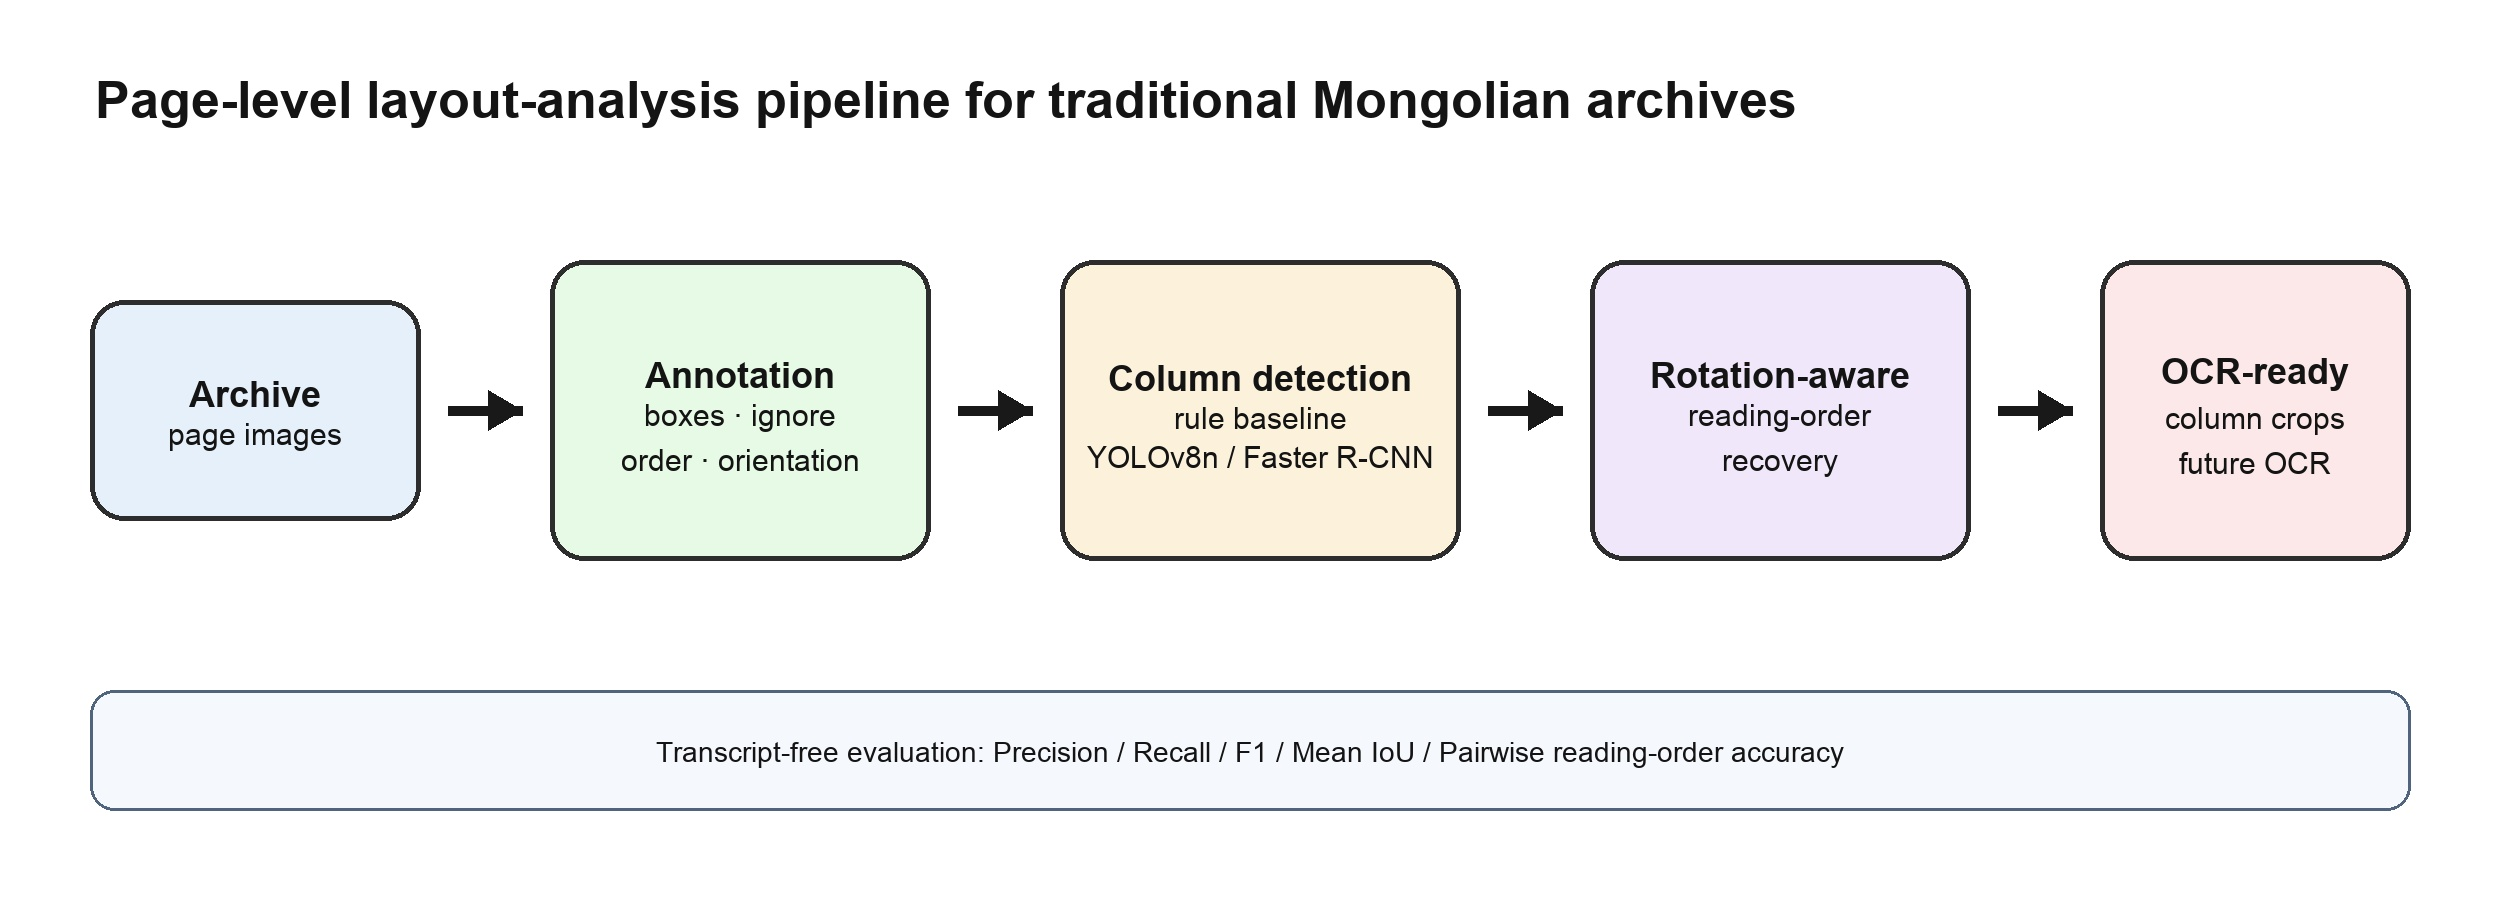
\includegraphics[width=\linewidth]{figures/page_layout_pipeline_overview.jpg}
\caption{Overview of the proposed page-level layout-analysis pipeline. The current study evaluates text-column detection and reading-order recovery without requiring expert text transcription.}
\label{fig:pipeline}
\end{figure}


\section{Related Work}
\subsection{Historical Document Layout Analysis}
Historical document image analysis has long treated segmentation as a prerequisite for reliable recognition. Likforman-Sulem et al.~\cite{likforman2007textline} review text-line segmentation methods for historical documents and emphasize that degradation, background noise, and handwriting variability make automatic page decomposition difficult. More recent dataset surveys also show that historical document collections vary widely in script, layout, degradation, and annotation granularity~\cite{nikolaidou2022survey}. For archival manuscripts, baseline and line detection datasets such as READ-BAD further highlight that realistic documents contain heterogeneous page layouts and challenging degradations~\cite{gruning2017readbad}. Large-scale multi-style historical benchmarks such as M5HisDoc~\cite{shi2023m5hisdoc} have advanced evaluation protocols for rotated, distorted, and resolution-varied historical inputs, though the focus remains on Chinese and printed documents. Traditional Mongolian recognition has been studied at word or character level, including large online handwriting resources such as MOLHW~\cite{pan2023molhw}, and hybrid CNN-Transformer architectures have been applied to Mongolian ancient document recognition~\cite{sun2023mongolian}. A dedicated dataset for Mongolian movable-type newspaper text recognition~\cite{lu2024mongolian} highlights the persistent data scarcity for Mongolian document analysis. Beyond script-specific resources, general-purpose historical document segmentation frameworks such as dhSegment~\cite{oliveira2018dhsegment} and large-scale historical manuscript datasets such as DIVA-HisDB~\cite{simistira2016diva} have enabled reproducible deep-learning benchmarks for medieval and early-modern manuscripts; competitions such as ICDAR RDCL~\cite{clausner2019icdar} further systematize the evaluation of complex historical layouts. Nevertheless, page-level layout analysis for \emph{handwritten} traditional Mongolian archives remains underexplored. Our task is closely related to historical segmentation, but the target units are vertical traditional Mongolian text columns rather than horizontal baselines or printed regions.

\subsection{Learning-Based Document Layout Detection}
Large-scale document-layout datasets and toolkits have accelerated learning-based layout analysis. PubLayNet introduced a large automatically annotated dataset for scientific-document layout analysis~\cite{zhong2019publaynet}, while DocLayNet provided diverse human annotations for modern document layouts~\cite{pfitzmann2022doclaynet}. LayoutParser demonstrated how deep-learning layout models can be organized into reusable document-analysis pipelines~\cite{shen2021layoutparser}. Recent YOLO-style document-layout models further show that one-stage detectors remain competitive for document analysis when adapted to layout-specific scale and aspect-ratio variation~\cite{deng2023yolo, zhao2024doclayout}. These resources mainly focus on modern printed or PDF-derived documents, whereas our archive pages are handwritten, vertically arranged, and affected by scanning rotation and cultural-heritage degradation. We therefore train a lightweight detector on our own page-level annotations instead of relying on off-the-shelf layout categories.

\subsection{Reading Order and Recognition-Ready Preprocessing}
Reading-order recovery is necessary for transforming detected regions into structured text. Quir\'os and Vidal~\cite{quiros2022reading} show that handwritten document understanding still requires explicit ordering beyond line recognition. Historical OCR frameworks such as OCR-D also treat layout analysis, segmentation, and recognition as separate but connected stages~\cite{neudecker2019ocrd}. Following this pipeline view, we evaluate text-column detection and reading order independently, and provide crop export for future recognition once expert column-level transcripts become available.

\section{Dataset and Annotation Protocol}
The current dataset contains 105 valid traditional Mongolian archive pages after removing Chinese handwritten archive pages and correcting pages with abnormal scan orientation. The split contains 43 training pages, 8 validation pages, an original 11-page test split, and a 43-page test-expansion split collected from additional archive folders. In earlier internal files the training split was named train\_unlabeled because it had no text transcripts; in this paper it refers to pages with layout annotations but without textual transcription. The annotations include 1538 valid text-column boxes and 199 ignored regions.

\begin{table}[t]
\centering
\scriptsize\setlength{\tabcolsep}{3pt}
\caption{Page-level annotation statistics.}
\label{tab:data_stats}
\begin{tabular}{lrrr}
\toprule
Split & Pages & TextColumn boxes & Ignored boxes \\
\midrule
train & 43 & 637 & 67 \\
val & 8 & 115 & 10 \\
original test & 11 & 152 & 45 \\
expanded test & 43 & 634 & 77 \\
\midrule
total & 105 & 1538 & 199 \\
\bottomrule
\end{tabular}
\end{table}


\begin{table}[t]
\centering
\scriptsize\setlength{\tabcolsep}{3pt}
\caption{Dataset distribution statistics computed over the 105-page corpus. Width, height, and bounding-box dimensions are measured in pixels.}
\label{tab:dataset_distribution}
\begin{tabular}{lrrrr}
\toprule
Quantity & Min & Max & Mean & Median \\
\midrule
Page width & 4830 & 7396 & 6596.8 & 6794 \\
Page height & 4830 & 9594 & 5436.2 & 4830 \\
Text columns per page & 1 & 25 & 14.6 & 16 \\
Ignore regions per page & 0 & 8 & 1.9 & 2 \\
Column-box width & 109 & 650 & 262.8 & 256 \\
Column-box height & 222 & 7883 & 3281.5 & 3503 \\
\bottomrule
\end{tabular}
\end{table}

In addition to the split-level counts in Table~\ref{tab:data_stats}, Table~\ref{tab:dataset_distribution} summarizes the spatial distribution of the current corpus. The pages are high-resolution scans with a median size of 6794 by 4830 pixels. The median page contains 16 valid text columns, while 64 of 105 pages contain at least one Ignore region and 21 pages required rotation or orientation correction before annotation. These statistics indicate that the dataset remains modest in size but is layout-dense, with substantial variation in column count, artifact frequency, and scan orientation.

\begin{table}[t]
\centering
\scriptsize\setlength{\tabcolsep}{3pt}
\caption{Inter-annotator agreement on the 5-page independent subset.}
\label{tab:iaa}
\begin{tabular}{lc}
\toprule
Metric & Value \\
\midrule
Box precision@0.5 & 0.929 \\
Box recall@0.5 & 0.788 \\
Box F1@0.5 & 0.852 \\
Mean matched IoU & 0.800 \\
Reading-order pairwise agreement & 0.677 \\
Ignore F1@0.5 & 0.286 \\
\bottomrule
\end{tabular}
\end{table}

Each non-ignored text column is annotated with a bounding box and reading-order index. Figure~\ref{fig:annotation} illustrates the annotation protocol on a representative page. Ignored regions are used for non-text artifacts, ambiguous fragments, or areas that should not be counted as false positives. Table~\ref{tab:iaa} reports the initial inter-annotator agreement on a 5-page subset. After the initial IAA analysis revealed low Ignore agreement, we refined the guideline to distinguish several recommended Ignore subtypes: seals or stamps, stains and background noise, page borders or scanning edges, non-target-language regions, ambiguous fragments, and unseparable artifact--text overlaps. These subtypes are used as annotation guidance rather than separate detector classes in the current experiments. Pages that were originally horizontal or upside down are relabeled after rotation so that the annotation coordinate system matches the displayed image.

\begin{table}[t]
\centering
\scriptsize\setlength{\tabcolsep}{3pt}
\caption{Recommended Ignore subtypes used to refine the annotation guideline. The current detector still evaluates a single Ignore category, but these subtypes clarify annotator decisions.}
\label{tab:ignore_subtypes}
\begin{tabular}{lp{0.62\textwidth}}
\toprule
Subtype & Description \\
\midrule
seal & Red seals or archive stamps that may be confused with text regions \\
stain/noise & Paper stains, ink bleed, background artifacts, or shadows \\
border/edge & Page borders, scan edges, black margins, or binding shadows \\
non-target language & Chinese or other non-target-language regions mixed into source folders \\
ambiguous fragment & Fragmentary strokes too incomplete to define a text column \\
overlap-unseparable & Artifact--text overlap that cannot be cleanly separated \\
\bottomrule
\end{tabular}
\end{table}


\begin{figure}[t]
\centering
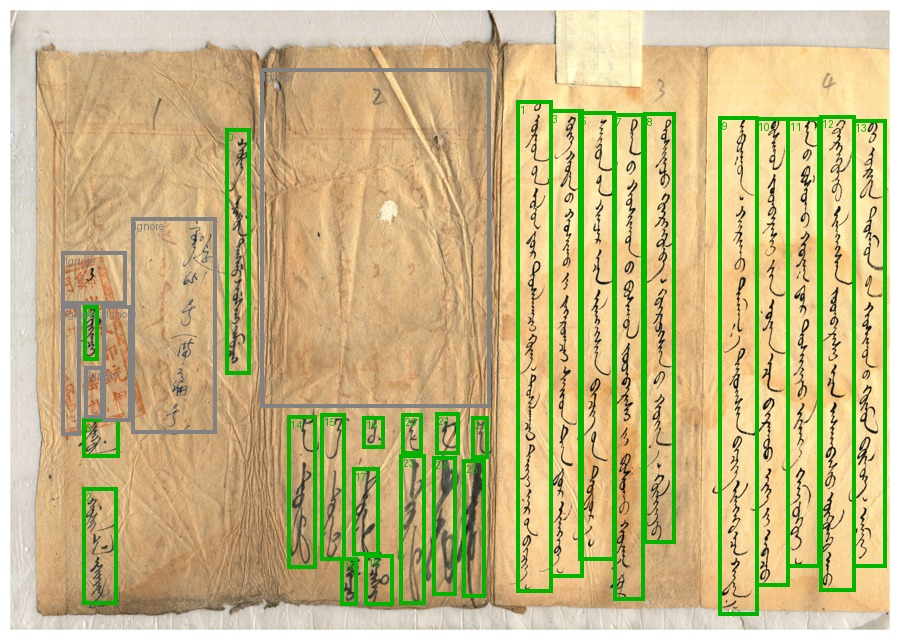
\includegraphics[width=0.75\linewidth]{figures/page_layout_annotation_example.jpg}
\caption{Example of the page-level annotation protocol. Green boxes indicate valid text columns with reading-order indices, while gray boxes indicate ignored regions that should not be counted as false positives.}
\label{fig:annotation}
\end{figure}

\section{Method}
\subsection{Rule-Based Baseline}
We evaluate three non-deep baselines before introducing YOLOv8n. The Sauvola-projection baseline applies local thresholding followed by vertical projection valley detection. The connected-component baseline groups foreground components into candidate column regions. The stronger rule-based baseline uses binarization, projection statistics, connected components, and heuristic filtering to identify vertical text-column candidates. The image is first converted to grayscale and binarized with an adaptive threshold. Vertical ink-density projections are then computed to obtain candidate column intervals. Connected components are used to suppress isolated stains and to estimate the vertical extent of each candidate. Finally, candidates are filtered by width, height coverage, and ink density, and overlapping candidates are merged before assigning a left-to-right reading order. This baseline is interpretable and does not require training data, but it is sensitive to paper noise, faint ink, and long-column over-merging. In the released code, all thresholds are fixed before test evaluation and the same ignore-region filtering protocol is used for both rule-based and learning-based predictions.

\subsection{YOLOv8n Column Detector}
We train a lightweight YOLOv8n detector~\cite{jocher2023yolov8} on page-level column boxes. YOLOv8n is selected as a practical baseline because it is fast, widely reproducible, and suitable for small custom detection datasets. The final detector is initialized from the public YOLOv8n weights and trained for 50 epochs with image size 960 and batch size 1. A batch size of 1 is used because full-page archive images are high resolution and the project was trained under limited local compute. The validation split is used only to select the confidence threshold. The main reported setting uses threshold 0.35, which gives the best validation F1 under the project-level IoU@0.5 matching metric. We do not claim architectural novelty in the detector itself; the methodological contribution of this version is the page-level annotation protocol, rotation-aware ordering, and transcript-free evaluation setting for traditional Mongolian archival pages.


\subsection{Column-Aware Post-processing Diagnostic}
To test whether explicit vertical-column priors improve detection, we additionally evaluate a simple column-aware post-processing variant for YOLO predictions. Candidate boxes are retained only if they satisfy validation-selected geometric constraints on confidence, aspect ratio, relative height, and relative width. Specifically, for a box with width $w$, height $h$, page width $W$, and page height $H$, the diagnostic filter keeps boxes satisfying $s\geq\theta$, $h/w\geq a_{\min}$, $h/H\geq r_h$, and $r_{w,\min}\leq w/W\leq r_{w,\max}$. The parameters are selected on the validation split by F1. This module is not used as the main result because the small validation set makes hand-tuned geometry priors prone to overfitting; it is included to clarify the trade-off between column priors, recall, and reading-order robustness.

\subsection{Faster R-CNN Detector Baseline}
To provide a second learned-detector reference point, we additionally fine-tune a Faster R-CNN MobileNetV3-FPN detector initialized from COCO-pretrained weights. The classification head is replaced with a two-class head for background and TextColumn. We fine-tune for 5 epochs with learning rate 0.0005 and image max-side 960. The confidence threshold is selected on the validation split, where 0.8 gives the best F1, and the selected threshold is then applied unchanged to the test split. This baseline provides a two-stage detector reference, but because the training schedule differs from YOLOv8n, the comparison should be interpreted diagnostically rather than as a compute-matched ranking.

\subsection{Document-Layout Detector Transfer Baselines}
We also examine two additional transfer baselines that are commonly associated with modern document-layout detection: RT-DETR and DocLayout-YOLO. RT-DETR is initialized from public pretrained weights and DocLayout-YOLO is initialized from a DocStructBench-pretrained checkpoint. For both baselines, the confidence threshold is selected only on the validation split before test evaluation. These models are included as supplementary transfer baselines because their pretraining domains are dominated by modern printed document layouts, which differ substantially from sparse, vertical, handwritten, and degraded archival columns. We report two training budgets for each: the initial 5-epoch diagnostic run (comparable to the Faster R-CNN budget) and a 50-epoch fair-budget run that matches YOLOv8n's training schedule. The 5-epoch results should be interpreted as preliminary diagnostic evidence; the 50-epoch results provide a more informative comparison of domain-transfer difficulty under comparable optimization effort.


\subsection{Training-Budget and Threshold Protocol}
Table~\ref{tab:training_protocol} summarizes the training and threshold-selection protocol. The primary learned-detector references are YOLOv8n and Faster R-CNN, both initialized from generic object-detection weights and adapted to the text-column class. RT-DETR and DocLayout-YOLO are reported separately to test whether modern document-layout priors transfer directly to this archive domain. All fixed-threshold test results use a threshold selected on the validation split, and no threshold is tuned on the test set.

\begin{table}[t]
\centering
\scriptsize\setlength{\tabcolsep}{3pt}
\caption{Training-budget and threshold-selection protocol. Transfer baselines are diagnostic rather than fully optimized comparisons because their architectures and pretraining domains differ substantially.}
\label{tab:training_protocol}
\begin{tabular}{p{0.28\linewidth}p{0.18\linewidth}ccp{0.22\linewidth}}
\toprule
Model & Init. domain & Epochs & Image size & Test threshold source \\
\midrule
YOLOv8n & COCO/general detection & 50 & 960 & validation F1, threshold 0.35 \\
Faster R-CNN MobileNetV3-FPN & COCO/general detection & 5 & 960 max-side & validation F1, threshold 0.80 \\
RT-DETR-L (diagnostic) & general detection & 5 & 640 & validation F1, threshold 0.10 \\
RT-DETR-L (fair budget) & general detection & 50 & 640 & validation F1, threshold 0.30 \\
DocLayout-YOLO (diagnostic) & DocStructBench layout & 5 & 1024 & validation F1, threshold 0.03 \\
DocLayout-YOLO (fair budget) & DocStructBench layout & 50 & 1024 & validation F1, threshold 0.15 \\
\bottomrule
\end{tabular}
\end{table}

\subsection{Rotation-Aware Reading-Order Recovery}
YOLO detections are unordered. For ordinary pages, detections are sorted by column center from left to right. For pages relabeled after 90-degree rotation, the order is reversed. Formally, for detections $b_i=(x_{1i},y_{1i},x_{2i},y_{2i})$, the column center is $c_i=(x_{1i}+x_{2i})/2$; detections are sorted by $c_i$ ascending for ordinary pages and descending for rotated pages. This step changes only the reading-order field and does not modify detection boxes. The rule is intentionally simple and transparent, and its limitations on multi-block or irregular layouts are discussed in Section~\ref{sec:discussion}. We note that the pairwise reading-order accuracy reported below is computed only on matched detection--ground-truth pairs, which makes it a proxy for the ordering module rather than a fully independent reading-order metric; a detector that misses complex columns may obtain optimistically high ordering scores. More sophisticated reading-order evaluation beyond pairwise agreement---such as edit distance or longest common subsequence between the full predicted and ground-truth column sequences---is left to future work, as is comparison with learned ordering methods~\cite{quiros2022reading}.

\subsection{Crop-Export Interface}
The pipeline exports both oracle crops from ground-truth boxes and detected crops from YOLO boxes. These crops can be passed to an existing OCR recognizer. However, because no expert column-level transcripts are currently available, CER/WER is not reported in this paper.

\section{Experiments}
\subsection{Evaluation Metrics}
Column detection is evaluated with greedy IoU@0.5 matching. Given true positives $TP$, false positives $FP$, and false negatives $FN$, we compute $P=TP/(TP+FP)$, $R=TP/(TP+FN)$, and $F1=2TP/(2TP+FP+FN)$. Mean IoU is averaged over matched prediction--ground-truth pairs. Reading-order accuracy is pairwise: for every pair of matched columns, we check whether the relative order of the two predictions is consistent with the relative order of their matched ground-truth columns. This order metric is computed only over matched boxes, so it is interpreted together with recall and full-page success. Predictions substantially overlapping ignored regions are not counted as false positives. In response to the strict page-level nature of archival processing, we also report complete detection rate, full-page success rate, Kendall's $\tau$, Spearman's $\rho$, and diagnostic stratified performance by page type. Complete detection requires all valid columns on a page to be matched with no false positives or false negatives; full-page success additionally requires perfect matched-pair reading order. To quantify the uncertainty caused by the still-modest expanded test set, we perform page-level bootstrap resampling with 1000 samples and report 95\% confidence intervals for P/R/F1. The AP values reported below are not COCO-style mAP; they are project-level confidence-sweep areas under the precision--recall curve, computed by sweeping detector confidence thresholds, applying the same ignore-region filtering, and aggregating matched and unmatched boxes over the evaluated pages.

\subsection{Main Results}
\begin{table}[t]
\centering
\scriptsize\setlength{\tabcolsep}{3pt}
\caption{Expanded 54-page test-set comparison under IoU@0.5 matching. RO Acc. denotes reading-order accuracy on matched columns.}
\label{tab:main_results}
\begin{tabular}{p{0.34\linewidth}ccccc}
\toprule
Method & Prec. & Rec. & F1 & Mean IoU & RO Acc. \\
\midrule
Heuristic column extraction & 0.694 & 0.753 & 0.722 & \textbf{0.881} & 0.882 \\
YOLOv8n + rotation-aware order & \textbf{0.936} & \textbf{0.821} & \textbf{0.875} & 0.756 & \textbf{0.887} \\
Faster R-CNN MobileNet + rotation-aware order & 0.924 & 0.816 & 0.866 & 0.744 & 0.870 \\
\bottomrule
\end{tabular}
\end{table}

Table~\ref{tab:main_results} summarizes the rule-based pipeline and two learning-based detectors on the expanded 54-page test set. The rule-based pipeline remains competitive in mean IoU on successfully matched boxes, but it produces more false positives and lower F1. YOLOv8n and Faster R-CNN are close in F1, with YOLOv8n slightly higher in this expanded evaluation. Given the modest test size and overlapping bootstrap intervals, this should be interpreted as a diagnostic comparison rather than evidence that one detector is clearly superior. To make the fixed-threshold evaluation auditable, Table~\ref{tab:main_counts} reports the underlying TP/FP/FN counts used to compute the main metrics.

Reading-order accuracy in Table~\ref{tab:main_results} is computed only on matched detections, so it should not be interpreted independently of recall. A method that misses many columns may still obtain a high ordering score on the easier subset of matched boxes. For this reason, we also report strict page-level success and complete-detection rates in Table~\ref{tab:enhanced_order}; full-page success remains low on the expanded test set, highlighting that the current system is not a fully automatic page-level solution.

\begin{table}[t]
\centering
\scriptsize\setlength{\tabcolsep}{3pt}
\caption{Raw detection counts for the main test-set comparison. All methods are evaluated against 786 non-ignored ground-truth text columns in the expanded 54-page test set.}
\label{tab:main_counts}
\begin{tabular}{lrrrr}
\toprule
Method & Pred. & TP & FP & FN \\
\midrule
Heuristic column extraction & 853 & 592 & 261 & 194 \\
YOLOv8n + rotation-aware order & 689 & 645 & 44 & 141 \\
Faster R-CNN MobileNet + rotation-aware order & 694 & 641 & 53 & 145 \\
\bottomrule
\end{tabular}
\end{table}

\begin{table}[t]
\centering
\scriptsize\setlength{\tabcolsep}{3pt}
\caption{Supplementary page-level and reading-order metrics on the expanded 54-page test set. Complete detection requires zero false positives and zero false negatives on a page; full-page success additionally requires perfect reading order among matched columns.}
\label{tab:enhanced_order}
\begin{tabular}{p{0.38\linewidth}ccc}
\toprule
Method & Complete det. & Full-page success & RO Acc. \\
\midrule
Heuristic column extraction & \textbf{0.148} & \textbf{0.148} & 0.882 \\
YOLOv8n + rotation-aware order & 0.111 & 0.074 & \textbf{0.887} \\
Faster R-CNN MobileNet + rotation-aware order & 0.111 & 0.093 & 0.870 \\
\bottomrule
\end{tabular}
\end{table}

The strict page-level metrics in Table~\ref{tab:enhanced_order} are intentionally more demanding than box-level F1. Full-page success remains low for all methods, because even one missed column or one extra column makes complete detection fail. This confirms that the current systems are useful as candidate crop generators, but still require human verification for page-level archival processing.

\begin{table}[t]
\centering
\scriptsize\setlength{\tabcolsep}{3pt}
\caption{Diagnostic stratified YOLOv8n performance on the original 11-page test split under IoU@0.5. These groups are not mutually exclusive; they diagnose sensitivity to page complexity, orientation, and ignored regions.}
\label{tab:stratified_yolo}
\begin{tabular}{lcccc}
\toprule
Group & Pages & Prec. & Rec. & F1 \\
\midrule
Few columns ($\leq$5) & 1 & 0.000 & 0.000 & 0.000 \\
Medium columns (6--15) & 5 & 0.943 & 0.579 & 0.717 \\
Many columns ($>$15) & 5 & 0.908 & 0.663 & 0.767 \\
Rotated pages & 2 & \textbf{1.000} & 0.357 & 0.526 \\
Pages with Ignore regions & 10 & 0.910 & 0.574 & 0.704 \\
No-Ignore page & 1 & 0.955 & \textbf{0.955} & \textbf{0.955} \\
\bottomrule
\end{tabular}
\end{table}

Table~\ref{tab:stratified_yolo} provides diagnostic observations rather than statistically stable subgroup conclusions, because several groups contain only one or two pages. On the original test split, the detector performs best on the no-ignore page and remains reasonably strong on many-column pages, but it is weak on the single few-column page and recall drops on rotated pages. This supports the failure analysis that fixed confidence thresholds and orientation-specific cases remain important targets for future work.

\begin{table}[t]
\centering
\scriptsize\setlength{\tabcolsep}{3pt}
\caption{Stratified YOLOv8n performance on the expanded 54-page test set by column count and Ignore presence, using the 43-page training model at threshold 0.35. With 54 test pages, the subgroup sizes are more informative than the original 11-page diagnostic.}
\label{tab:stratified_expanded}
\begin{tabular}{lcccc}
\toprule
Group & Pages & Prec. & Rec. & F1 \\
\midrule
Few columns ($\leq$5) & 4 & 0.900 & 0.600 & 0.720 \\
Medium columns (6--15) & 22 & 0.869 & 0.727 & 0.791 \\
Many columns ($>$15) & 28 & 0.936 & 0.880 & \textbf{0.907} \\
Pages with Ignore regions & 7 & 0.924 & 0.718 & 0.808 \\
No-Ignore pages & 47 & 0.914 & 0.837 & 0.874 \\
\bottomrule
\end{tabular}
\end{table}

Table~\ref{tab:stratified_expanded} confirms the pattern observed in the smaller diagnostic table: many-column pages are best served, few-column pages remain challenging (F1 = 0.720 on 4 pages), and pages with Ignore regions show a modest performance penalty relative to clean pages (0.808 vs. 0.874). The expanded stratification is more informative than the original 11-page version because the few-column group now contains 4 pages instead of 1 and the medium/many groups are large enough to provide meaningful subgroup comparisons.

\begin{table}[t]
\centering
\scriptsize\setlength{\tabcolsep}{3pt}
\caption{Transfer-detector baselines on the original 11-page test split. The 5-epoch results use the same short budget as Faster R-CNN; the 50-epoch results match YOLOv8n's training budget for fairer comparison.}
\label{tab:transfer_baselines}
\begin{tabular}{p{0.34\linewidth}ccccc}
\toprule
Method & Prec. & Rec. & F1 & Mean IoU & RO Acc. \\
\midrule
RT-DETR-L 5ep + rotation-aware order & 0.032 & 0.270 & 0.058 & 0.632 & 0.847 \\
RT-DETR-L 50ep + rotation-aware order & 0.183 & 0.132 & 0.153 & 0.622 & 1.000 \\
DocLayout-YOLO 5ep + rotation-aware order & 0.046 & 0.031 & 0.037 & 0.572 & 0.000 \\
DocLayout-YOLO 50ep + rotation-aware order & 0.635 & 0.572 & 0.602 & 0.709 & 0.900 \\
\bottomrule
\end{tabular}
\end{table}

Table~\ref{tab:transfer_baselines} reports detector-transfer attempts at two training budgets. Under the 5-epoch short budget, both RT-DETR and DocLayout-YOLO are very weak, producing many low-quality candidate regions. Extending the training budget to 50 epochs substantially changes the picture for DocLayout-YOLO, which improves from F1 = 0.037 to 0.602. This suggests that the DocStructBench layout priors do contain transferable features for sparse vertical archive columns, but they require extended domain adaptation to become practically useful. RT-DETR also improves (0.058 $\to$ 0.153) but remains far below YOLOv8n and Faster R-CNN even after 50 epochs. Both still underperform the heuristic baseline (F1 = 0.507 on the original test), confirming that off-the-shelf modern document-layout priors do not transfer directly to this domain without substantial architectural or pretraining adaptation. The 5-epoch results alone would underestimate DocLayout-YOLO's potential by a factor of 16$\times$ in F1, underscoring that fair-budget comparison is essential for reliable transfer diagnosis. These transfer baselines are evaluated on the 11-page original test split rather than the expanded 54-page test due to computational resource limits; extending the fair-budget evaluation to the expanded test is planned for future work.


\begin{table}[t]
\centering
\scriptsize\setlength{\tabcolsep}{3pt}
\caption{Supplementary strict-localization comparison on the original 11-page test split at IoU@0.75. The stricter threshold penalizes boundary errors more heavily.}
\label{tab:iou75}
\begin{tabular}{p{0.34\linewidth}ccccc}
\toprule
Method & Prec. & Rec. & F1 & Mean IoU & RO Acc. \\
\midrule
Heuristic column extraction & 0.322 & 0.447 & 0.375 & \textbf{0.901} & \textbf{1.000} \\
YOLOv8n + rotation-aware order & \textbf{0.579} & \textbf{0.434} & \textbf{0.496} & 0.826 & \textbf{1.000} \\
Faster R-CNN MobileNet + rotation-aware order & 0.352 & 0.289 & 0.318 & 0.828 & \textbf{1.000} \\
\bottomrule
\end{tabular}
\end{table}


\begin{table}[t]
\centering
\scriptsize\setlength{\tabcolsep}{3pt}
\caption{Page-level bootstrap 95\% confidence intervals on the expanded 54-page test set.}
\label{tab:bootstrap_ci}
\begin{tabular}{p{0.34\linewidth}ccc}
\toprule
Method & Precision 95\% CI & Recall 95\% CI & F1 95\% CI \\
\midrule
Heuristic column extraction & [0.599, 0.793] & [0.688, 0.813] & [0.643, 0.800] \\
YOLOv8n + rotation-aware order & [0.907, 0.960] & [0.769, 0.865] & [0.834, 0.906] \\
Faster R-CNN MobileNet + rotation-aware order & [0.897, 0.948] & [0.762, 0.862] & [0.830, 0.897] \\
\bottomrule
\end{tabular}
\end{table}


\subsection{Effect of Training Set Size}
We also monitored YOLOv8n performance as additional page-level annotations were added. Table~\ref{tab:train_size} reports project-level metrics on the original 11-page test split under the same IoU@0.5 matching protocol. Increasing the training set from 7 to 43 pages improves test recall from 0.388 to 0.717 and F1 from 0.532 to 0.820 in this split, suggesting that additional layout annotation is likely useful; larger evaluation splits are needed before drawing stable scaling conclusions.

\begin{table}[t]
\centering
\scriptsize\setlength{\tabcolsep}{3pt}
\caption{YOLOv8n project-level performance on the original 11-page test split with different numbers of annotated training pages. These metrics use the same IoU@0.5 matching protocol as Table~\ref{tab:main_results}.}
\label{tab:train_size}
\begin{tabular}{lccccc}
\toprule
Training pages & Test Prec. & Test Rec. & Test F1 & Mean IoU & RO Acc. \\
\midrule
7 & 0.843 & 0.388 & 0.532 & 0.719 & 1.000 \\
20 & 0.875 & 0.691 & 0.772 & 0.748 & 0.900 \\
43 & \textbf{0.956} & \textbf{0.717} & \textbf{0.820} & \textbf{0.770} & \textbf{0.900} \\
\bottomrule
\end{tabular}
\end{table}

\subsection{Threshold Sensitivity}
Table~\ref{tab:threshold} reports validation threshold sensitivity for YOLOv8n; the final threshold is selected on the validation split and then reused unchanged for the expanded test evaluation.
\begin{table}[t]
\centering
\scriptsize\setlength{\tabcolsep}{3pt}
\caption{Validation threshold sensitivity for YOLOv8n on the 8-page validation split. The final threshold is selected on the validation split and reused unchanged for the expanded test evaluation.}
\label{tab:threshold}
\begin{tabular}{lccc}
\toprule
Threshold & Val Prec. & Val Rec. & Val F1 \\
\midrule
0.25 & 0.746 & 0.787 & 0.766 \\
0.30 & 0.812 & 0.759 & 0.785 \\
0.35 & \textbf{0.876} & 0.722 & \textbf{0.792} \\
0.40 & 0.873 & 0.639 & 0.738 \\
\bottomrule
\end{tabular}
\end{table}


\begin{table}[t]
\centering
\scriptsize\setlength{\tabcolsep}{3pt}
\caption{Project-level confidence-sweep area under the precision--recall curve on the original 11-page test split. These values are reported separately from standard COCO-style AP because they use the project matching and ignore-region filtering protocol. These AP diagnostics are retained for the original test split and are not used as the main expanded-test result.}
\label{tab:project_ap}
\begin{tabular}{lcc}
\toprule
Method & AP@0.50 & AP@0.75 \\
\midrule
YOLOv8n + rotation-aware order & \textbf{0.921} & \textbf{0.399} \\
Faster R-CNN MobileNet + rotation-aware order & 0.700 & 0.097 \\
\bottomrule
\end{tabular}
\end{table}



\begin{table}[t]
\centering
\scriptsize\setlength{\tabcolsep}{3pt}
\caption{Diagnostic column-aware YOLO post-processing on the original 11-page test split. The parameters are selected on validation F1. The result is not used as the main setting because the hand-tuned prior does not robustly dominate the validation-selected YOLO setting and lowers reading-order accuracy on the original diagnostic test split.}
\label{tab:column_aware_diag}
\begin{tabular}{lcccccc}
\toprule
Setting & Split & Prec. & Rec. & F1 & Mean IoU & RO Acc. \\
\midrule
Main YOLO threshold 0.35 & test & 0.956 & 0.717 & 0.820 & 0.770 & 0.900 \\
Recall-oriented threshold 0.30 & test & 0.937 & 0.776 & \textbf{0.849} & 0.761 & 0.818 \\
Column-aware prior filter & val & \textbf{0.929} & 0.791 & 0.854 & 0.779 & 0.875 \\
Column-aware prior filter & test & 0.949 & 0.730 & 0.825 & 0.760 & \textbf{0.818} \\
\bottomrule
\end{tabular}
\end{table}

Table~\ref{tab:column_aware_diag} shows that explicit vertical-column priors can improve validation F1 and slightly change original-test detection metrics, but they do not robustly dominate the simpler validation-selected YOLO setting: the recall-oriented threshold gives higher original-test F1, while the column-aware prior lowers reading-order accuracy. We therefore keep the simpler validation-selected YOLO threshold as the main setting and treat column-aware filtering as a diagnostic experiment rather than an improvement claim. This result indicates that future column-aware modeling should be learned or regularized more robustly instead of relying only on hand-tuned geometric thresholds.

\subsection{Qualitative Analysis}
The qualitative examples in Fig.~\ref{fig:qualitative} show that YOLOv8n reduces many false columns caused by noise and page borders, while also recovering more degraded columns than the rule-based method. Remaining errors are concentrated on few-column pages, pages with severe over-merging, and ambiguous noisy regions.

\begin{figure}[!htbp]
\centering
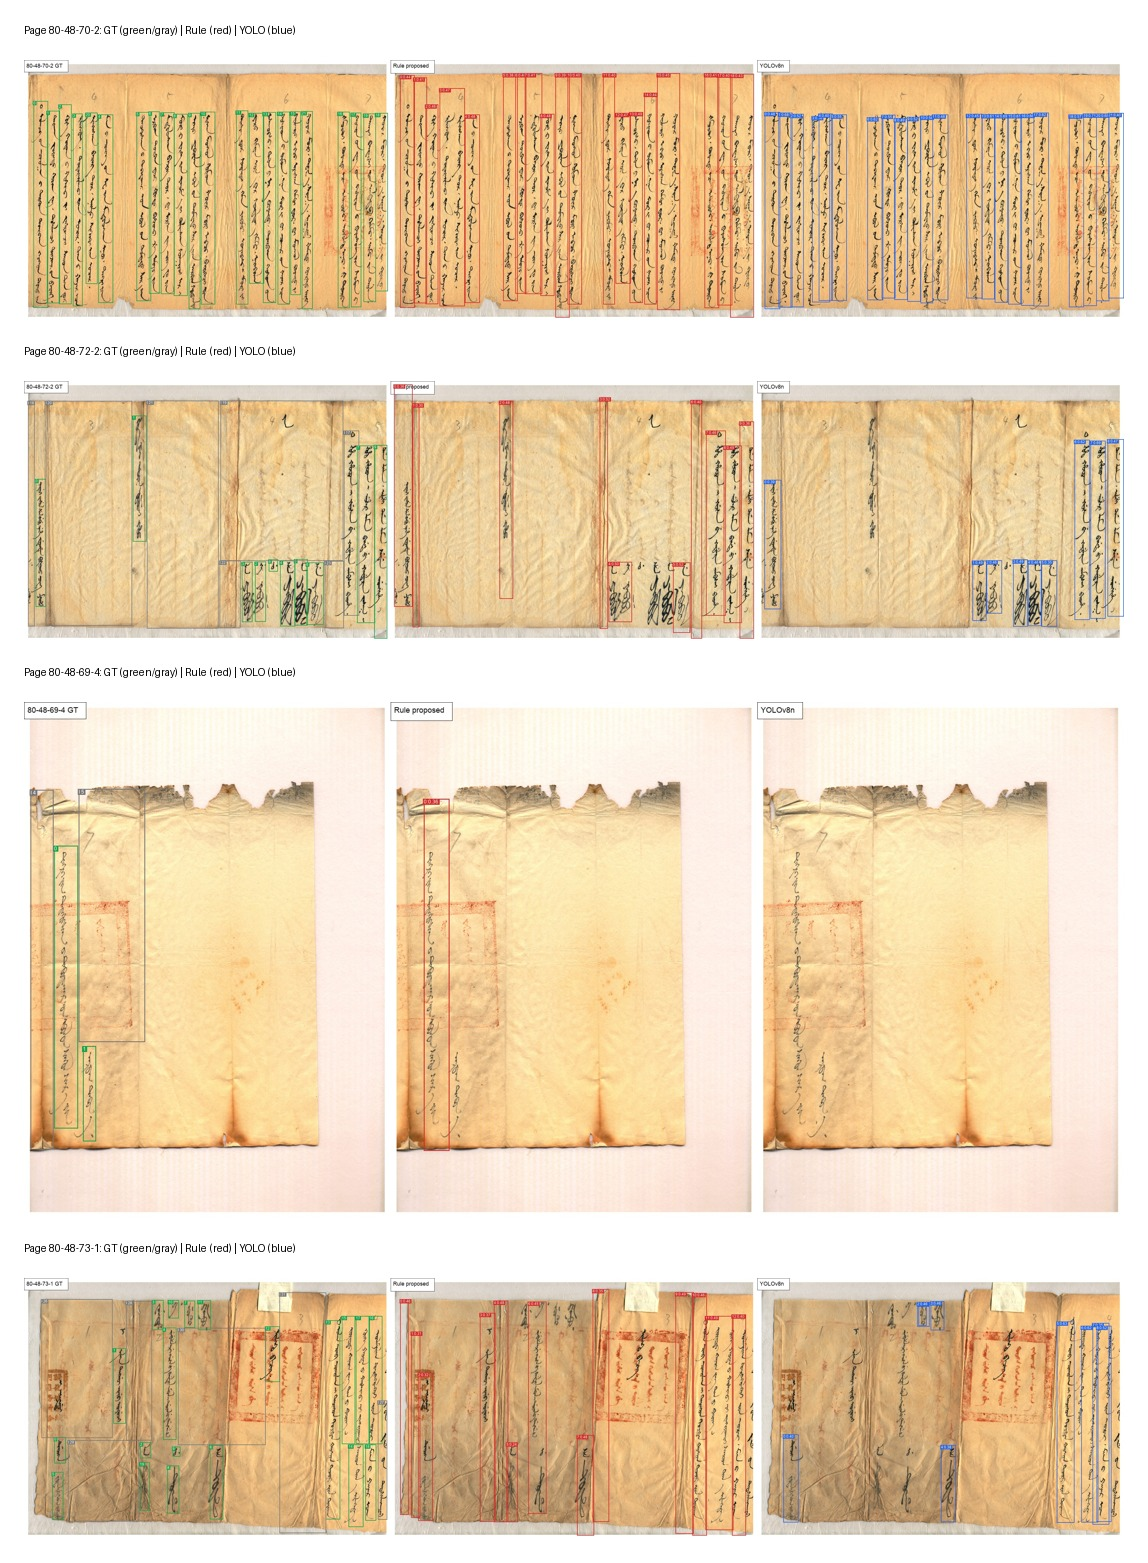
\includegraphics[width=\linewidth]{figures/page_layout_qualitative_failure_montage.jpg}
\caption{Representative page-level comparisons. Each row shows ground truth, rule-based predictions, and YOLOv8n predictions. Green denotes valid text columns, gray denotes ignored regions, red denotes rule-based detections, and blue denotes YOLO detections.}
\label{fig:qualitative}
\end{figure}




\subsection{Ablation of Ignore Filtering and Rotation-Aware Ordering}
Table~\ref{tab:ablation} evaluates two post-processing choices at the selected confidence threshold 0.35. On the corrected test labels, ignore-region filtering does not suppress any YOLO predictions, so detection F1 is unchanged across the four settings. Rotation-aware ordering also leaves detection F1 unchanged, but on the original small test split the x-sorted order happens to give slightly higher reading-order accuracy than the rotation-aware heuristic. This means the ordering rule should still be treated as a diagnostic heuristic rather than a fully solved component.

\begin{table}[t]
\centering
\scriptsize\setlength{\tabcolsep}{3pt}
\caption{Ablation of ignore-region filtering and rotation-aware reading order at score threshold 0.35 on the original 11-page test split. Removed denotes predictions suppressed because they overlap an Ignore region.}
\label{tab:ablation}
\begin{tabular}{lcccccc}
\toprule
Configuration & Prec. & Rec. & F1 & RO Acc. & FP/FN & Removed \\
\midrule
Full: ignore + rotation-aware order & \textbf{0.956} & 0.717 & \textbf{0.820} & 0.900 & 5 / 43 & 0 \\
w/o rotation-aware order & \textbf{0.956} & 0.717 & \textbf{0.820} & \textbf{1.000} & 5 / 43 & 0 \\
w/o ignore filtering & \textbf{0.956} & 0.717 & \textbf{0.820} & 0.900 & 5 / 43 & 0 \\
w/o both & \textbf{0.956} & 0.717 & \textbf{0.820} & \textbf{1.000} & 5 / 43 & 0 \\
\bottomrule
\end{tabular}
\end{table}


\subsection{Runtime Analysis}
Table~\ref{tab:runtime} reports inference time on the original 11-page test split using local CPU execution. The rule-based pipeline requires 1.84 seconds per page on average, while YOLOv8n requires 0.19 seconds per page at image size 960 after a one-image warm-up. Faster R-CNN is slightly faster in this local CPU measurement. These timings should be interpreted as implementation-specific diagnostics rather than general speed rankings, because batching, preprocessing, hardware, and framework versions can change the relative runtime.

\begin{table}[t]
\centering
\scriptsize\setlength{\tabcolsep}{3pt}
\caption{Runtime on the original 11-page test split under local CPU execution.}
\label{tab:runtime}
\begin{tabular}{lccc}
\toprule
Method & Device & Mean s/page & Median s/page \\
\midrule
Heuristic column extraction & CPU & 1.843 & 1.729 \\
YOLOv8n + rotation-aware order & CPU & 0.193 & 0.196 \\
Faster R-CNN MobileNet + rotation-aware order & CPU & \textbf{0.168} & \textbf{0.162} \\
\bottomrule
\end{tabular}
\end{table}

\subsection{Failure Analysis}
Across the expanded evaluation and the retained diagnostic analyses, the remaining errors can be grouped into five categories. First, few-column pages are sensitive to a fixed confidence threshold; for example, some valid columns may be filtered out at threshold 0.35. Second, rule-based methods tend to over-merge multiple short text segments into long boxes, producing simultaneous false positives and false negatives under IoU matching. Third, rotated or upside-down scans require explicit orientation handling, otherwise the box order may be geometrically valid but semantically reversed. Fourth, red seals, paper stains, and edge shadows still introduce ambiguous regions that require either ignore annotations or stronger artifact modeling. Fifth, the diagnostic column-aware post-processing in Table~\ref{tab:column_aware_diag} shows that hand-tuned vertical-column priors can overfit validation statistics and reduce test recall, motivating learned or data-adaptive column priors in future work.

\section{Discussion and Limitations}
\label{sec:discussion}
This study intentionally focuses on layout analysis rather than transcription-based OCR accuracy. To assess annotation reliability, we also asked an independent annotator to label a 5-page subset. The resulting agreement is moderate to strong for text-column boxes (F1@0.5 = 0.852) and mean matched IoU (0.800), while reading-order agreement is lower (0.677), reflecting the ambiguity of some multi-column pages. Ignore-region agreement remains weaker and is now explicitly treated as a limitation rather than a polished result; the refined Ignore subtypes in Table~\ref{tab:ignore_subtypes} are intended to improve future annotation consistency. Future annotation work should include more double-labeled pages, adjudicated disagreement examples, and visual examples that clarify subtype boundaries for seals, stains, borders, and ambiguous fragments. Since expert transcription of handwritten traditional Mongolian columns is unavailable, reporting CER/WER would be misleading. The current pipeline is nevertheless crop-export-ready: it can export oracle and automatically detected column crops and connect them to a recognizer once reliable transcripts are added.

Important limitations remain. A fixed confidence threshold can miss few-column pages; rule-based post-processing may over-merge multi-segment columns; and pages with seals or strong background noise still require more robust artifact handling. The current corpus has 105 pages and the expanded test set has 54 pages, which reduces but does not eliminate statistical uncertainty; subgroup analyses are still diagnostic only and should not be read as stable population-level conclusions. A further concern is that all hyper-parameters---including confidence thresholds, geometric priors for the column-aware diagnostic, and the threshold for ignore-region filtering---are selected on a validation split of only 8 pages. With such a small validation set, the selected values may overfit to the validation distribution, and re-selecting them on a different random split could yield different conclusions. Future work should therefore consider k-fold cross-validation, leave-one-archive-folder-out evaluation, or pre-registration of threshold choices before test evaluation to strengthen reproducibility. Ignore-region agreement in the 5-page IAA subset is lower than box agreement, suggesting that even the refined Ignore subtype guideline requires more examples and annotator training before it can be considered mature. The original-test AP results in Table~\ref{tab:project_ap} and the stricter IoU@0.75 results in Table~\ref{tab:iou75} show that boundary precision remains challenging, especially under high-overlap evaluation. Even the expanded test set is still modest, so the bootstrap intervals in Table~\ref{tab:bootstrap_ci} should be interpreted as an honest uncertainty estimate rather than a final large-scale benchmark. The transfer baselines in Table~\ref{tab:transfer_baselines} also suggest that modern document-layout detectors do not automatically solve this historical archive setting, but the unequal training budgets in Table~\ref{tab:training_protocol} mean that these results should be interpreted as diagnostic transfer tests rather than final optimized comparisons; stronger domain adaptation, column-aware pretraining, and fairer compute-matched retraining remain necessary. Faster R-CNN was not exhaustively optimized in this study; its close F1 to YOLOv8n and slightly faster local runtime suggest that two-stage detection deserves further investigation under a compute-matched protocol. Because full-page success remains low, future work should also measure human correction time and downstream OCR effects from exported crops rather than relying only on box-level metrics. Future work will add a small expert-transcribed subset, enabling oracle-crop and detected-crop CER/WER evaluation. Full retraining at different image sizes remains future work.

\section{Conclusion}
We presented a pilot low-resource page-level layout-analysis protocol for traditional Mongolian historical archives under a realistic condition where expert text transcription is unavailable. The work's primary contributions to the traditional Mongolian archival document community are: (i) a clearly defined page-level annotation protocol with Ignore subtypes suitable for real archive degradations, (ii) an auditable evaluation package with bootstrap-based uncertainty quantification on an expanded 54-page test set, and (iii) evidence that a small set of layout annotations can train a lightweight detector that achieves higher F1 than a classical heuristic baseline (0.875 vs.~0.722) under the reported protocol. For the broader document analysis community, the study provides a diagnostic comparison framework demonstrating that modern document-layout transfer baselines require fair training budgets and domain adaptation before conclusions about their inapplicability are drawn; our 50-epoch retraining of DocLayout-YOLO raised its F1 from 0.037 to 0.602. However, full-page success remains low (0.074 for YOLOv8n) and no new detector architecture or learned reading-order module is proposed; therefore the present system should be viewed as a candidate crop generator and diagnostic evaluation package rather than a fully automatic page-level OCR preprocessing solution.


\section*{Data Availability}
The non-image research artifacts produced in this study can be shared with reviewers or released publicly when allowed by project policy. The archive images themselves are subject to institutional access constraints and require authorized access. To maximize auditability despite image restrictions, the following materials are prepared for release: (i) the full annotation schema (English and Chinese) and 105-page split manifest with page identifiers, (ii) prediction files (JSON) for all reported tables, (iii) Python scripts for metric computation (greedy IoU matching, reading-order evaluation, bootstrap resampling, stratified analysis) with documented command-line entry points, (iv) training protocol documentation including random seed (20260513), optimizer (SGD with momentum 0.937), learning rate schedule (cosine, initial 0.01), data augmentation defaults (mosaic 1.0, hsv augmentation, no custom freeze layers), NMS configuration (default ultralytics YOLOv8n), and environment versions (Python~3.9, PyTorch~2.8, ultralytics~8.4) to enable independent replication given authorized images. Metric recomputation from the shared annotations and prediction files is fully reproducible without retraining or GPU access.

\section*{Author Contributions}
Lanying Liang: Conceptualization, Data Curation, Writing -- Original Draft. Yuefeng Liu: Methodology, Software, Validation, Writing -- Review \& Editing, Supervision.

\section*{Ethics Statement}
This study uses historical archive images for document analysis and digital preservation. No personal intervention or modern human-subject experiment is involved. The work does not attempt to infer sensitive attributes of living individuals. The archive images may contain historical seals and institutional markings; these are treated as layout artifacts (Ignore regions) and are not used to extract or publish personal identifiers. All example figures shown in this paper have been reviewed and approved for publication by the hosting archive institution.

\section*{Funding}
This work was supported by the National Natural Science Foundation of China (Grant No. 62341604), the Science and Technology Project of Inner Mongolia Autonomous Region Archives Bureau (Grant No. 2022-36), the China Scholarship Council (Grant No. 202408150080), and the General Project of the 14th Five-Year Plan for Educational Science of Inner Mongolia Autonomous Region (Grant No. NGJGH2025013).

\clearpage


\begin{thebibliography}{99}

\bibitem{likforman2007textline}
L. Likforman-Sulem, A. Zahour, and B. Taconet, ``Text line segmentation of historical documents: a survey,'' \emph{International Journal on Document Analysis and Recognition}, vol. 9, pp. 123--138, 2007. doi: 10.1007/s10032-006-0023-z.

\bibitem{nikolaidou2022survey}
K. Nikolaidou, M. Seuret, H. Mokayed, and M. Liwicki, ``A survey of historical document image datasets,'' \emph{International Journal on Document Analysis and Recognition}, vol. 25, pp. 305--338, 2022. doi: 10.1007/s10032-022-00405-8.

\bibitem{gruning2017readbad}
T. Gr\"uning, R. Labahn, M. Diem, F. Kleber, and S. Fiel, ``READ-BAD: A new dataset and evaluation scheme for baseline detection in archival documents,'' arXiv:1705.03311, 2017.

\bibitem{zhong2019publaynet}
X. Zhong, J. Tang, and A. J. Yepes, ``PubLayNet: largest dataset ever for document layout analysis,'' in \emph{Proc. International Conference on Document Analysis and Recognition}, 2019, pp. 1015--1022. doi: 10.1109/ICDAR.2019.00166.

\bibitem{pfitzmann2022doclaynet}
B. Pfitzmann, C. Auer, M. Dolfi, A. S. Nassar, and P. W. J. Staar, ``DocLayNet: A large human-annotated dataset for document-layout analysis,'' in \emph{Proc. ACM SIGKDD International Conference on Knowledge Discovery and Data Mining}, 2022. doi: 10.1145/3534678.3539043.

\bibitem{shen2021layoutparser}
Z. Shen, R. Zhang, M. Dell, B. C. G. Lee, J. Carlson, and W. Li, ``LayoutParser: A unified toolkit for deep learning based document image analysis,'' in \emph{Document Analysis and Recognition -- ICDAR 2021}, LNCS 12821, pp. 131--146, 2021. doi: 10.1007/978-3-030-86549-8\_9.

\bibitem{quiros2022reading}
L. Quir\'os and E. Vidal, ``Reading order detection on handwritten documents,'' \emph{Neural Computing and Applications}, vol. 34, pp. 9593--9611, 2022. doi: 10.1007/s00521-022-06948-5.

\bibitem{neudecker2019ocrd}
C. Neudecker, K. Baierer, M. Federbusch, M. Boenig, K.-M. W\"urzner, V. Hartmann, and E. Herrmann, ``OCR-D: An end-to-end open source OCR framework for historical printed documents,'' in \emph{Proc. DATeCH2019}, 2019, pp. 53--58. doi: 10.1145/3322905.3322917.


\bibitem{pan2023molhw}
Y. Pan, D. Fan, H. Wu, and D. Teng, ``A new dataset for Mongolian online handwritten recognition,'' \emph{Scientific Reports}, vol. 13, article 26, 2023. doi: 10.1038/s41598-022-27267-8.

\bibitem{deng2023yolo}
Q. Deng, M. Ibrayim, A. Hamdulla, and C. Zhang, ``The YOLO model that still excels in document layout analysis,'' \emph{Signal, Image and Video Processing}, vol. 18, no. 2, pp. 1539--1548, 2024. doi: 10.1007/s11760-023-02838-y.

\bibitem{zhao2024doclayout}
Z. Zhao, H. Kang, B. Wang, and C. He, ``DocLayout-YOLO: Enhancing document layout analysis through diverse synthetic data and global-to-local adaptive perception,'' arXiv:2410.12628, 2024.

\bibitem{jocher2023yolov8}
G. Jocher, A. Chaurasia, and J. Qiu, ``Ultralytics YOLOv8,'' software, version 8.0.0, 2023. Available: \url{https://github.com/ultralytics/ultralytics}.

\bibitem{shi2023m5hisdoc}
Y. Shi, C. Liu, D. Peng, C. Jian, et al., ``M5HisDoc: A large-scale multi-style Chinese historical document analysis benchmark,'' in \emph{Proc. NeurIPS}, 2023.

\bibitem{sun2023mongolian}
S. Sun, H. Wei, and Y. Wang, ``A hybrid approach using convolution and transformer for Mongolian ancient documents recognition,'' in \emph{Proc. ICONIP}, 2023.

\bibitem{lu2024mongolian}
M. Lu, F. Bao, H. Zhang, and G. Gao, ``The image and ground truth dataset of Mongolian movable-type newspapers for text recognition,'' \emph{IJDAR}, 2024.

\bibitem{oliveira2018dhsegment}
S. Ares Oliveira, B. Seguin, and F. Kaplan, ``dhSegment: A generic deep-learning approach for document segmentation,'' in \emph{Proc. ICFHR}, 2018, pp. 7--12.

\bibitem{simistira2016diva}
F. Simistira, M. Seuret, N. Eichenberger, A. Garz, M. Liwicki, and R. Ingold, ``DIVA-HisDB: A precisely annotated large dataset of challenging medieval manuscripts,'' in \emph{Proc. ICFHR}, 2016, pp. 471--476.

\bibitem{clausner2019icdar}
C. Clausner, A. Antonacopoulos, and S. Pletschacher, ``ICDAR2019 competition on recognition of documents with complex layouts---RDCL2019,'' in \emph{Proc. ICDAR}, 2019, pp. 1521--1526.

\end{thebibliography}


\end{document}
